
\documentclass{tp_um}
\makeatletter
%--------------------------------------------------------------------------------

\usepackage[frenchb]{babel}

\usepackage{amsmath}
\usepackage{amsbsy}
\usepackage{amsfonts}
\usepackage{amssymb}
\usepackage{amscd}
\usepackage{amsthm}
\usepackage{mathtools}
\usepackage{eurosym}
\usepackage{nicefrac}

\usepackage{latexsym}
\usepackage[a4paper,hmargin=20mm,vmargin=25mm]{geometry}
\usepackage{dsfont}
\usepackage[utf8]{inputenc}
\usepackage[T1]{fontenc}

\usepackage{multicol}
\usepackage[inline]{enumitem}
%\setlist{nosep}
\setlist[itemize,1]{,label=$-$}

\usepackage{sectsty}
%\sectionfont{}
\allsectionsfont{\normalfont\sffamily\bfseries\normalsize}

\usepackage{graphicx}
\usepackage{tikz}

\usepackage{pgfplots}
\usepgfplotslibrary{fillbetween}
\pgfplotsset{compat=newest}
%\usepgfplotslibrary{external} 
%\tikzexternalize[prefix=./output_latex/]
%\DeclareSymbolFont{RalphSmithFonts}{U}{rsfs}{m}{n}
%\DeclareSymbolFontAlphabet{\mathscr}{RalphSmithFonts}
%\def\mathcal#1{{\mathscr #1}}

\newcounter{zut}
\setcounter{zut}{1}
\newcommand{\exo}[1]{\noindent {\sffamily\bfseries Exercice~\thezut. #1} \
		   \addtocounter{zut}{1}}



\providecommand{\abs}[1]{\left|#1\right|}
\providecommand{\norm}[1]{\left\Vert#1\right\Vert}
\providecommand{\U}{\mathcal{U}}
\providecommand{\R}{\mathbb{R}}
\providecommand{\Cc}{\mathcal{C}}
\providecommand{\reg}[1]{\mathcal{C}^{#1}}
\providecommand{\1}{\mathds{1}}
\providecommand{\N}{\mathbb{N}}
\providecommand{\Z}{\mathbb{Z}}
\providecommand{\E}{\mathbb{E}}
\providecommand{\p}{\partial}
\providecommand{\one}{\mathds{1}}
\renewcommand{\P}{\mathbb{P}}


%Operateur
\providecommand{\abs}[1]{\left\lvert#1\right\rvert}
\providecommand{\sabs}[1]{\lvert#1\rvert}
\providecommand{\babs}[1]{\bigg\lvert#1\bigg\rvert}
\providecommand{\norm}[1]{\left\lVert#1\right\rVert}
\providecommand{\bnorm}[1]{\bigg\lVert#1\bigg\rVert}
\providecommand{\snorm}[1]{\lVert#1\rVert}
\providecommand{\prs}[1]{\left\langle #1\right\rangle}
\providecommand{\sprs}[1]{\langle #1\rangle}
\providecommand{\bprs}[1]{\bigg\langle #1\bigg\rangle}

\DeclareMathOperator{\deet}{Det}
\DeclareMathOperator{\vol}{Vol}
\DeclareMathOperator{\aire}{Aire}
\DeclareMathOperator{\hess}{Hess}
\DeclareMathOperator{\var}{Var}

%------------------------------------------------------------------------------
\DeclareUnicodeCharacter{00A0}{~}
\makeatother


\newcommand{\miniscule}{\@setfontsize\miniscule{5}{6}}
%-----------------------------------------------------------------------------




	\title{\Large \sffamily\bfseries Représentation de fonctions}
\ue{HLMA410}

%-----------------------------------------------------------------------------
\begin{document}

\maketitle

\section{Représentation de fonctions}

%\exo{} Déterminer et représenter le domaine de définition des fonctions suivantes: \\
%\begin{enumerate*}
	%\item	$f(x,y)= \frac{\sqrt{-y+x^2}}{y}$,
	%\item   $f(x,y) = \frac{\ln(y)}{\sqrt{x-y}}$,
%\item   $f(x,y) = \ln(x+y)$,
%\item  $f(x,y,z) = \frac{\ln(x^2+1)}{yz} $.
%\end{enumerate*}

%\bigskip

%\bigskip

\exo{} Associer à chaque fonction ($1$ à $6$) une surface ($a$ à $f$) et des courbes de niveau (I à VI).
\begin{multicols}{3}
\begin{enumerate}
    \item $(x,y) \mapsto e^x \cos(y)$
	\item $(x,y) \mapsto \frac{1}{1+x^2+y^2}$
	\item $(x,y) \mapsto \sin(x) - \sin(y)$
	\item $(x,y) \mapsto (x-y)^2$
	\item $(x,y) \mapsto \frac{x-y}{1+x^2+y^2}$
	\item $(x,y) \mapsto \sin(\abs{x} + \abs{y})$
\end{enumerate}
\end{multicols}

\begin{tabular}{ccc}
	\begin{tikzpicture}[scale=.6]
		\begin{axis}[xlabel=$x$,ylabel=$y$,zmin=-2,zmax=4,xtick=\empty,ytick=\empty,ztick=\empty]
			\addplot3[surf,domain=-9:9,samples=40,opacity=.8] gnuplot {sin(abs(x) + abs(y))};
		\end{axis}
	\end{tikzpicture}	&
	\begin{tikzpicture}[scale=.6]
		\begin{axis}[,xlabel=$x$,ylabel=$y$,xtick=\empty,ytick=\empty,ztick=\empty ]
			\addplot3[surf,opacity=.8] gnuplot {(x-y)**2};%{ (x^2)^.5 + (y^2)^.5 };
		\end{axis}
	\end{tikzpicture}&
	\begin{tikzpicture}[scale=.6]
		\begin{axis}[,xlabel=$x$,ylabel=$y$,xtick=\empty,ytick=\empty,ztick=\empty ]
			\addplot3[surf,samples=50,opacity=.8] gnuplot {1/(1+x**2 + y**2)};
		\end{axis}
	\end{tikzpicture}\\ $a$& $b$&$c$ \\

	\begin{tikzpicture}[scale=.6]
		\begin{axis}[,xlabel=$x$,ylabel=$y$,xtick=\empty,ytick=\empty,ztick=\empty ]
			\addplot3[surf,samples=50,opacity=.8] gnuplot {(x-y)/(1+x**2 + y**2)};
		\end{axis}
\end{tikzpicture}&
	\begin{tikzpicture}[scale=.6]
		\begin{axis}[,xlabel=$x$,ylabel=$y$,zmin=-2,zmax=4,xtick=\empty,ytick=\empty,ztick=\empty ]
			\addplot3[surf,domain=-9:9,samples=40,opacity=.8] gnuplot {sin(x) - sin(y)};
		\end{axis}
	\end{tikzpicture}&
	\begin{tikzpicture}[scale=.6]
		\begin{axis}[,xlabel=$x$,ylabel=$y$,xtick=\empty,ytick=\empty,ztick=\empty ]
			\addplot3[surf,domain=-2:2,y domain=-9:9,samples=50,opacity=.8] gnuplot {cos(y) * exp(x)};
		\end{axis}
	\end{tikzpicture} 
\\ $d$ & $e$ &$f$ \\
\end{tabular}
\bigskip

\begin{tabular}{ccc}
\begin{tikzpicture}[scale=.6]
	\begin{axis}[xlabel=$x$,ylabel=$y$,zmin=-2,zmax=2,view={0}{90},xtick=\empty,ytick=\empty,ztick=\empty ,]
		\addplot3[domain=-9:9,contour gnuplot={number=10, labels=false},samples=40] gnuplot {sin(abs(x) + abs(y))};
	\end{axis}
\end{tikzpicture}
&
\begin{tikzpicture}[scale=.6]
		\begin{axis}[,xlabel=$x$,ylabel=$y$,view={0}{90},xtick=\empty,ytick=\empty,ztick=\empty ]
			\addplot3[contour gnuplot={number=19, labels=false},domain=-2:2,y domain=-9:9,samples=50] gnuplot {cos(y) * exp(x)};
		\end{axis} 
\end{tikzpicture}
&
\begin{tikzpicture}[scale=.6]
	\begin{axis}[xlabel=$x$,ylabel=$y$,view={0}{90},xtick=\empty,ytick=\empty,ztick=\empty ,]
		\addplot3[contour gnuplot={number=19, labels=false},samples=50] gnuplot {1/(1+x**2 + y**2)};
	\end{axis}
\end{tikzpicture}
\\ I & II & III \\
\begin{tikzpicture}[scale=.6]
		\begin{axis}[,xlabel=$x$,ylabel=$y$,view={0}{90},xtick=\empty,ytick=\empty,ztick=\empty ]
			\addplot3[contour gnuplot={number=19, labels=false},samples=50] gnuplot {(x-y)/(1+x**2 + y**2)};
		\end{axis}
\end{tikzpicture}
&
\begin{tikzpicture}[scale=.6]
		\begin{axis}[,xlabel=$x$,ylabel=$y$,view={0}{90},xtick=\empty,ytick=\empty,ztick=\empty ]
			\addplot3[,domain=-9:9,samples=40,contour gnuplot={number=15, labels=false}] gnuplot {sin(x) - sin(y)};
		\end{axis}
\end{tikzpicture}
&
\begin{tikzpicture}[scale=.6]
	\begin{axis}[xlabel=$x$,ylabel=$y$,view={0}{90},xtick=\empty,ytick=\empty,ztick=\empty ,]
		\addplot3[contour gnuplot={number=40, labels=false}] gnuplot {(x-y)**2};
	\end{axis}
\end{tikzpicture}
\\ IV & V & VI\\
\end{tabular}
\bigskip

\newpage

\exo{} Déterminer et représenter les courbes de niveau des fonctions suivantes: \\
\begin{multicols}{3}
\begin{enumerate}
	\item	$f(x,y) = \deet(\begin{psmallmatrix}
			1\\2
		\end{psmallmatrix}, \begin{psmallmatrix}
			x \\ y
	\end{psmallmatrix}) $, 
	\item $f(x,y) = \prs{\begin{psmallmatrix}
			1\\2
		\end{psmallmatrix}, \begin{psmallmatrix}
			x \\ y
	\end{psmallmatrix}}$, 
	\item $f(x,y) = (x-1)^2+y^2$, 
	\item $f(x,y) = e^{y-x^2}$, 
	\item $f(x,y) = y - \cos(x)$,
    \item $f(x,y) = \snorm{\begin{psmallmatrix}
			x \\ y
	\end{psmallmatrix}}_1$, 
    \item $f(x,y) = \snorm{\begin{psmallmatrix}
			x \\ y
	\end{psmallmatrix}}_2$, 
    \item $f(x,y) = \snorm{\begin{psmallmatrix}
			x \\ y
	\end{psmallmatrix}}_\infty$. 
\end{enumerate}
\end{multicols}
%\exo{} Associer à chaque fonction ($1$ à $12$) une surface ($a$ à $\ell$) et des courbes de niveau (I à XII).
%\begin{multicols}{4}
%\begin{enumerate}
	%\item $\sin(xy)$ 
	%\item $\sin(x) - \sin(y)$
	%\item $\frac{1}{1+x^2+y^2}$
	%\item $\abs{x}+\abs{y}$
	%\item $e^x \cos(y)$
	%\item $\frac{x-y}{1+x^2+y^2}$
	%\item $(x-y)^2$
	%\item $\sin(x-y)$
	%\item $(1-x^2)(1-y)$
	%\item $\abs{xy}$
	%\item $ \sin(\abs{x} + \abs{y})$
	%\item $ (x^2 -y^2)^2$
%\end{enumerate}
%\end{multicols}

%\begin{tabular}{ccc}
	%\begin{tikzpicture}[scale=.7]
		%\begin{axis}[xlabel=$x$,ylabel=$y$,xtick=\empty,ytick=\empty,ztick=\empty ]
			%\addplot3[surf] gnuplot {abs(y*x)};%{ (x^2)^.5 + (y^2)^.5 };
		%\end{axis}
	%\end{tikzpicture}&
	%\begin{tikzpicture}[scale=.7]
		%\begin{axis}[,xlabel=$x$,ylabel=$y$,xtick=\empty,ytick=\empty,ztick=\empty ]
			%\addplot3[surf] gnuplot {(x-y)**2};%{ (x^2)^.5 + (y^2)^.5 };
		%\end{axis}
	%\end{tikzpicture}&
	%\begin{tikzpicture}[scale=.7]
		%\begin{axis}[,xlabel=$x$,ylabel=$y$,xtick=\empty,ytick=\empty,ztick=\empty ]
			%\addplot3[surf,samples=50] gnuplot {1/(1+x**2 + y**2)};
		%\end{axis}
	%\end{tikzpicture}\\ $a$& $b$&$c$ \\
	%\begin{tikzpicture}[scale=.7]
		%\begin{axis}[xlabel=$x$,ylabel=$y$,zmin=-2,zmax=4,xtick=\empty,ytick=\empty,ztick=\empty]
			%\addplot3[surf,domain=-9:9,samples=40] gnuplot {sin(abs(x) + abs(y))};
		%\end{axis}
	%\end{tikzpicture}&
	%\begin{tikzpicture}[scale=.7]
		%\begin{axis}[,xlabel=$x$,ylabel=$y$,xtick=\empty,ytick=\empty,ztick=\empty ]
			%\addplot3[surf] gnuplot {(x**2 - y**2)**2};
		%\end{axis}
	%\end{tikzpicture}&
	%\begin{tikzpicture}[scale=.7]
		%\begin{axis}[,xlabel=$x$,ylabel=$y$,xtick=\empty,ytick=\empty,ztick=\empty ]
			%\addplot3[surf] gnuplot {abs(x) + abs(y)};
		%\end{axis}
	%\end{tikzpicture}\\ $d$ & $e$ &$f$ \\
	%\begin{tikzpicture}[scale=.7]
		%\begin{axis}[xlabel=$x$,ylabel=$y$,zmin=-2,zmax=4,xtick=\empty,ytick=\empty,ztick=\empty]
			%\addplot3[surf] gnuplot {sin(x-y)};
		%\end{axis}
	%\end{tikzpicture}&
	%\begin{tikzpicture}[scale=.7]
		%\begin{axis}[,xlabel=$x$,ylabel=$y$,xtick=\empty,ytick=\empty,ztick=\empty ]
			%\addplot3[surf,domain=-4:4] gnuplot {(1-x**2)*(1-y**1)};%{ (x^2)^.5 + (y^2)^.5 };
		%\end{axis}
	%\end{tikzpicture}&
	%\begin{tikzpicture}[scale=.7]
		%\begin{axis}[,xlabel=$x$,ylabel=$y$,xtick=\empty,ytick=\empty,ztick=\empty ]
			%\addplot3[surf,samples=50] gnuplot {(x-y)/(1+x**2 + y**2)};
		%\end{axis}
	%\end{tikzpicture}\\ $g$ & $h$ & $i$ \\
	%\begin{tikzpicture}[scale=.7]
		%\begin{axis}[xlabel=$x$,ylabel=$y$,zmin=-2,zmax=4,xtick=\empty,ytick=\empty,ztick=\empty ]
			%\addplot3[surf,domain=-3:3,samples=40] gnuplot {sin(x*y)};
		%\end{axis}
	%\end{tikzpicture}&
	%\begin{tikzpicture}[scale=.7]
		%\begin{axis}[,xlabel=$x$,ylabel=$y$,zmin=-2,zmax=4,xtick=\empty,ytick=\empty,ztick=\empty ]
			%\addplot3[surf,domain=-9:9,samples=40] gnuplot {sin(x) - sin(y)};
		%\end{axis}
	%\end{tikzpicture}&
	%\begin{tikzpicture}[scale=.7]
		%\begin{axis}[,xlabel=$x$,ylabel=$y$,xtick=\empty,ytick=\empty,ztick=\empty ]
			%\addplot3[surf,domain=-2:2,y domain=-9:9,samples=50] gnuplot {cos(y) * exp(x)};
		%\end{axis}
	%\end{tikzpicture} \\ $j$ & $k$ & $\ell$
%\end{tabular}
%\bigskip

%\begin{tabular}{ccc}
%\begin{tikzpicture}[scale=.7]
	%\begin{axis}[xlabel=$x$,ylabel=$y$,view={0}{90},xtick=\empty,ytick=\empty,ztick=\empty ,]
		%\addplot3[contour gnuplot={levels={5,0,10,50,100,200}, labels=false},samples=50] gnuplot {(x**2 - y**2)**2};
	%\end{axis}
%\end{tikzpicture}
%&
%\begin{tikzpicture}[scale=.7]
	%\begin{axis}[xlabel=$x$,ylabel=$y$,zmin=-2,zmax=2,view={0}{90},xtick=\empty,ytick=\empty,ztick=\empty ,]
		%\addplot3[domain=-9:9,contour gnuplot={number=10, labels=false},samples=40] gnuplot {sin(abs(x) + abs(y))};
	%\end{axis}
%\end{tikzpicture}
%&
%\begin{tikzpicture}[scale=.7]
		%\begin{axis}[xlabel=$x$,ylabel=$y$,view={0}{90},zmin=-2,zmax=2,xtick=\empty,ytick=\empty,ztick=\empty ]
			%\addplot3[contour gnuplot={number=10, labels=false},domain=-3:3,samples=40] gnuplot {sin(x*y)};
		%\end{axis}
%\end{tikzpicture}
%\\ I & II & III \\
%\begin{tikzpicture}[scale=.7]
		%\begin{axis}[xlabel=$x$,ylabel=$y$,view={0}{90},zmin=-2,zmax=2,xtick=\empty,ytick=\empty,ztick=\empty]
			%\addplot3[contour gnuplot={number=19, labels=false}] gnuplot {sin(x-y)};
		%\end{axis}
%\end{tikzpicture}
%&
%\begin{tikzpicture}[scale=.7]
	%\begin{axis}[xlabel=$x$,ylabel=$y$,view={0}{90},xtick=\empty,ytick=\empty,ztick=\empty ,]
		%\addplot3[contour gnuplot={number=40, labels=false}] gnuplot {(x-y)**2};
	%\end{axis}
%\end{tikzpicture}
%&
%\begin{tikzpicture}[scale=.7]
		%\begin{axis}[,xlabel=$x$,ylabel=$y$,view={0}{90},xtick=\empty,ytick=\empty,ztick=\empty ]
			%\addplot3[contour gnuplot={number=19, labels=false},domain=-2:2,y domain=-9:9,samples=50] gnuplot {cos(y) * exp(x)};
		%\end{axis} 
%\end{tikzpicture}
%\\ IV & V & VI\\
%\begin{tikzpicture}[scale=.7]
	%\begin{axis}[xlabel=$x$,ylabel=$y$,view={0}{90},xtick=\empty,ytick=\empty,ztick=\empty ,]
		%\addplot3[contour gnuplot={number=19, labels=false},] {abs(x) + abs(y)};
	%\end{axis}
%\end{tikzpicture}
%&
%\begin{tikzpicture}[scale=.7]
		%\begin{axis}[,xlabel=$x$,ylabel=$y$,view={0}{90},xtick=\empty,ytick=\empty,ztick=\empty ]
			%\addplot3[,domain=-9:9,samples=40,contour gnuplot={number=15, labels=false}] gnuplot {sin(x) - sin(y)};
		%\end{axis}
%\end{tikzpicture}
%&
%\begin{tikzpicture}[scale=.7]
	%\begin{axis}[xlabel=$x$,ylabel=$y$,view={0}{90},xtick=\empty,ytick=\empty,ztick=\empty ,]
		%\addplot3[contour gnuplot={number=19, labels=false},samples=50] gnuplot {1/(1+x**2 + y**2)};
	%\end{axis}
%\end{tikzpicture}
%\\ VII & VIII & IX \\
%\begin{tikzpicture}[scale=.7]
	%\begin{axis}[xlabel=$x$,ylabel=$y$,view={0}{90},,xtick=\empty,ytick=\empty,ztick=\empty]
		%\addplot3[contour gnuplot={number=19, labels=false}]  {abs(y*x)};
	%\end{axis}
%\end{tikzpicture}
%&
%\begin{tikzpicture}[scale=.7]
		%\begin{axis}[,xtick=\empty,ytick=\empty,ztick=\empty ,xlabel=$x$,ylabel=$y$,xlabel=$x$,ylabel=$y$,view={0}{90}]
			%\addplot3[contour gnuplot={number=19, labels=false}] gnuplot {(1-x**2)*(1-y)};%{ (x^2)^.5 + (y^2)^.5 };
		%\end{axis}
%\end{tikzpicture}
%&
%\begin{tikzpicture}[scale=.7]
		%\begin{axis}[,xlabel=$x$,ylabel=$y$,view={0}{90},xtick=\empty,ytick=\empty,ztick=\empty ]
			%\addplot3[contour gnuplot={number=19, labels=false},samples=50] gnuplot {(x-y)/(1+x**2 + y**2)};
		%\end{axis}
%\end{tikzpicture}
%\\ X & XI & XII
%\end{tabular}
%\bigskip

%\exo{(Cartographie)} Voici les courbes de niveau d'une carte topographique. 
%\begin{center}
	%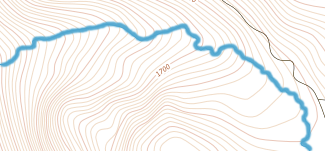
\includegraphics[height=3.7cm]{./levelsets.png}
%\end{center}
%Dans quel sens la rivière coule-t-elle ?
%%\begin{enumerate}
	%%\item Est-ce une crète (une ``bosse'') ou un talweg (un ``creux'') ?
	%%\item Dans quel sens la rivière coule-t-elle ?
%%\end{enumerate}
%\bigskip

\newpage

\exo{}
On pose $r = \sqrt{x^2 + y^2}$ (distance à l'origine). On s'intéresse au cas particulier $f(x,y) = g (r(x,y))$.
\begin{enumerate}
	\item Donner les équations des fonctions polynomiales (de degré 4) en double puits dont les graphes sont les suivants:
		\begin{center}
			\begin{tikzpicture}[scale=.5]
				\begin{axis}[xlabel=$x$,ylabel=$y$,ymax=5,grid=major]
                    \addplot[blue, very thick, samples=200] {(x^2-1)*(x^2-4)};
				\end{axis}
			\end{tikzpicture}
			\begin{tikzpicture}[scale=.5]
				\begin{axis}[xlabel=$x$,ylabel=$y$,ymin=-1,ymax=5,grid=major,]
					\addplot[blue, very thick, samples=200] {x^4 -x^2};
				\end{axis}
			\end{tikzpicture}
		\end{center}
	\item En déduire l'expression des fonctions dont le graphe sont les surfaces de révolutions suivantes:
		\begin{center}
			%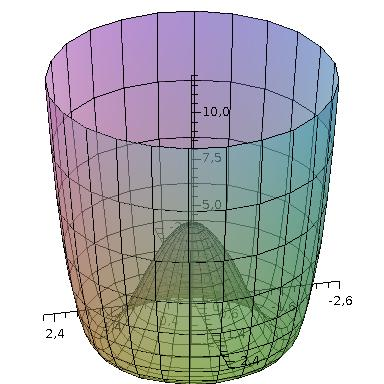
\includegraphics[height=2.4cm]{./revol1.png}
			%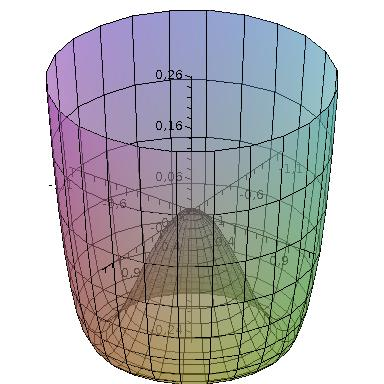
\includegraphics[height=2.4cm]{./revol2.png}
\begin{tikzpicture}
    \begin{axis}[xlabel=$x$,ylabel=$y$,grid=major,view={20}{40},z buffer=sort, data cs=polar]
        \addplot3 [surf, domain=0:360, domain y=-2.3:2.3,samples=30, samples y=40, opacity=.3]
        {(y^2 -1)*(y^2 -4)};
    \end{axis}
  \end{tikzpicture}  
\begin{tikzpicture}
    \begin{axis}[xlabel=$x$,ylabel=$y$,grid=major,view={20}{40},z buffer=sort, data cs=polar]
        \addplot3 [surf, domain=0:360, domain y=-1.2:1.2,samples=30, samples y=40, opacity=.3]
        {y^4 - y^2 )};
    \end{axis}
  \end{tikzpicture}  

		\end{center}
\end{enumerate}

\newpage

\exo{} Associer à chaque champ de vecteurs suivants sa représentation graphique:
\begin{multicols}{3}
	\begin{enumerate}
		\item $f(x,y) =(-x,-y)$
		\item $f(x,y) =(y,-x)$
		\item $f(x,y) =\frac{(1, x-y)}{\sqrt{1+(x-y)^2}}$
		\item $f(x,y) =(e^{-0.3x^2},0)$
		\item $f(x,y) =(.8,.5)$
		\item $f(x,y) =(-x,\ln(y^2+1))$
	\end{enumerate}
\end{multicols}

\begin{tabular}{ccc}
	\def\length{sqrt(1+(x-y)^2)}
	\begin{tikzpicture}[scale=.6]
		\begin{axis}[,xtick=\empty,ytick=\empty,ztick=\empty ,xlabel=$x$,ylabel=$y$,xlabel=$x$,ylabel=$y$,domain=-3:3, view={0}{90}]
			\addplot3[blue, quiver={u={1/(\length)}, v={(x-y)/(\length)}, scale arrows=.7}, -stealth,samples=10] {0};
		\end{axis}
	\end{tikzpicture}
	&
	\begin{tikzpicture}[scale=.6]
		\begin{axis}[,xtick=\empty,ytick=\empty,ztick=\empty ,xlabel=$x$,ylabel=$y$,xlabel=$x$,ylabel=$y$,domain=-3:3, view={0}{90}]
			\addplot3[blue, quiver={u={-x}, v={-y}, scale arrows=0.25}, -stealth,samples=10] {0};
		\end{axis}
	\end{tikzpicture}
	&
	\begin{tikzpicture}[scale=.6]
		\begin{axis}[,xtick=\empty,ytick=\empty,ztick=\empty ,xlabel=$x$,ylabel=$y$,xlabel=$x$,ylabel=$y$,domain=-3:3, view={0}{90}]
			\addplot3[blue, quiver={u={-x}, v={ln(y^2+1)}, scale arrows=0.15}, -stealth,samples=15] {0};
		\end{axis}
	\end{tikzpicture}
	\\$a$&$b$& $c$ \\
	\begin{tikzpicture}[scale=.6]
		\begin{axis}[,xtick=\empty,ytick=\empty,ztick=\empty ,xlabel=$x$,ylabel=$y$,xlabel=$x$,ylabel=$y$,domain=-3:3, view={0}{90}]
			\addplot3[blue, quiver={u={.8}, v={.5}, scale arrows=.8}, -stealth,samples=10] {0};
		\end{axis}
	\end{tikzpicture}
	&
	\begin{tikzpicture}[scale=.6]
		\begin{axis}[,xtick=\empty,ytick=\empty,ztick=\empty ,xlabel=$x$,ylabel=$y$,xlabel=$x$,ylabel=$y$,domain=-3:3, view={0}{90}]
			\addplot3[blue, quiver={u={exp(-.3*x^2)}, v={0}, scale arrows=.5}, -stealth,samples=10,samples y=15] {0};
		\end{axis}
	\end{tikzpicture}
	&
	\begin{tikzpicture}[scale=.6]
		\begin{axis}[,xtick=\empty,ytick=\empty,ztick=\empty ,xlabel=$x$,ylabel=$y$,xlabel=$x$,ylabel=$y$,domain=-3:3, view={0}{90}]
			\addplot3[blue, quiver={u={y}, v={-x}, scale arrows=.5}, -stealth,samples=10] {0};
		\end{axis}
	\end{tikzpicture}
	\\ $d$ & $e$ & $f$
\end{tabular}
\end{document}
